\documentclass[tcc]{subfiles}

\begin{document}

\chapter{Materials and methods}
\label{ch:methods}

\section{The instrumentation}
The engine was instrumented to provide measurements of the following:
\begin{compactitem}
    \item Ambient pressure
    \item Ambient temperature
    \item Ambient relative humidity
    \item Fuel flow
    \item Air mass flow
    \item Static pressure at compressor exit
    \item Temperature at compressor exit
    \item Temperature at turbine entry
    \item Pressure at turbine exit
    \item Temperature at turbine exit
    \item \gls{EGT}
    \item Shaft rotational speed
    \item Thrust
\end{compactitem}

All pressures are measured by pressure transducers, and temperatures by type K thermocouples. 
Air mass flow is measured through an specially designed admission nozzle. 
Thrust is measured from a load cell installed in the engine mounts.
For a specification of each sensor used, refer to \cref{app:instrumentation}.

All sensors are read though an acquisition card 
model DAQ USB-6009 manufactured by National Instruments .
Every signal was amplified up to this board's operational range (-10V to 10V). 
The data acquired is then processed by a program developed in-house.%
\footnote{this program is available at \todo{put program on github}}

\section{The test bench}

The test bench used for this project was designed and built by Frederico Bolsoni at the \gls{ALFALAB}.
It was made so that its weight is at least ten times the engine thrust 
 and its natural frequencies are separated from those of the engine \cite{bolsoni}.
The test bench is shown in \cref{fig:test_bench}.

\begin{figure}[p]
    \centering
    \caption{Test bench}
    \label{fig:test_bench}
    \begin{subfigure}{.49\textwidth}
        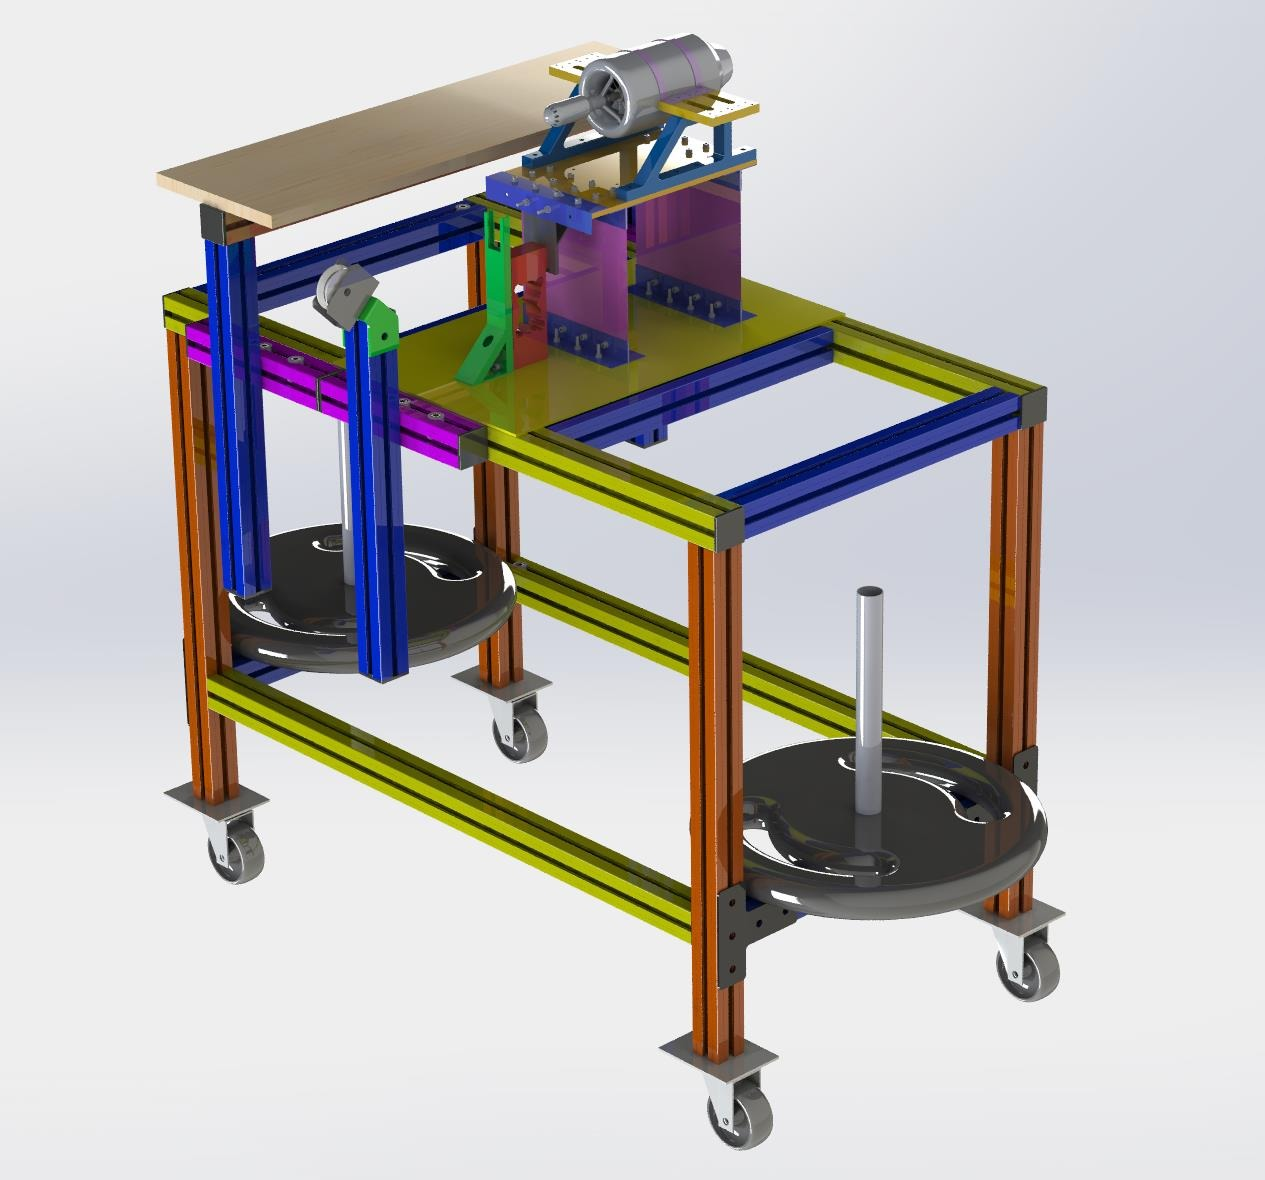
\includegraphics[width=.9\textwidth]{fig/test_bench_rendering.jpg}
        \caption{\acs{CAD} rendering}
        \label{fig:test_bench!rendering}
    \end{subfigure}
    \begin{subfigure}{.49\textwidth}
        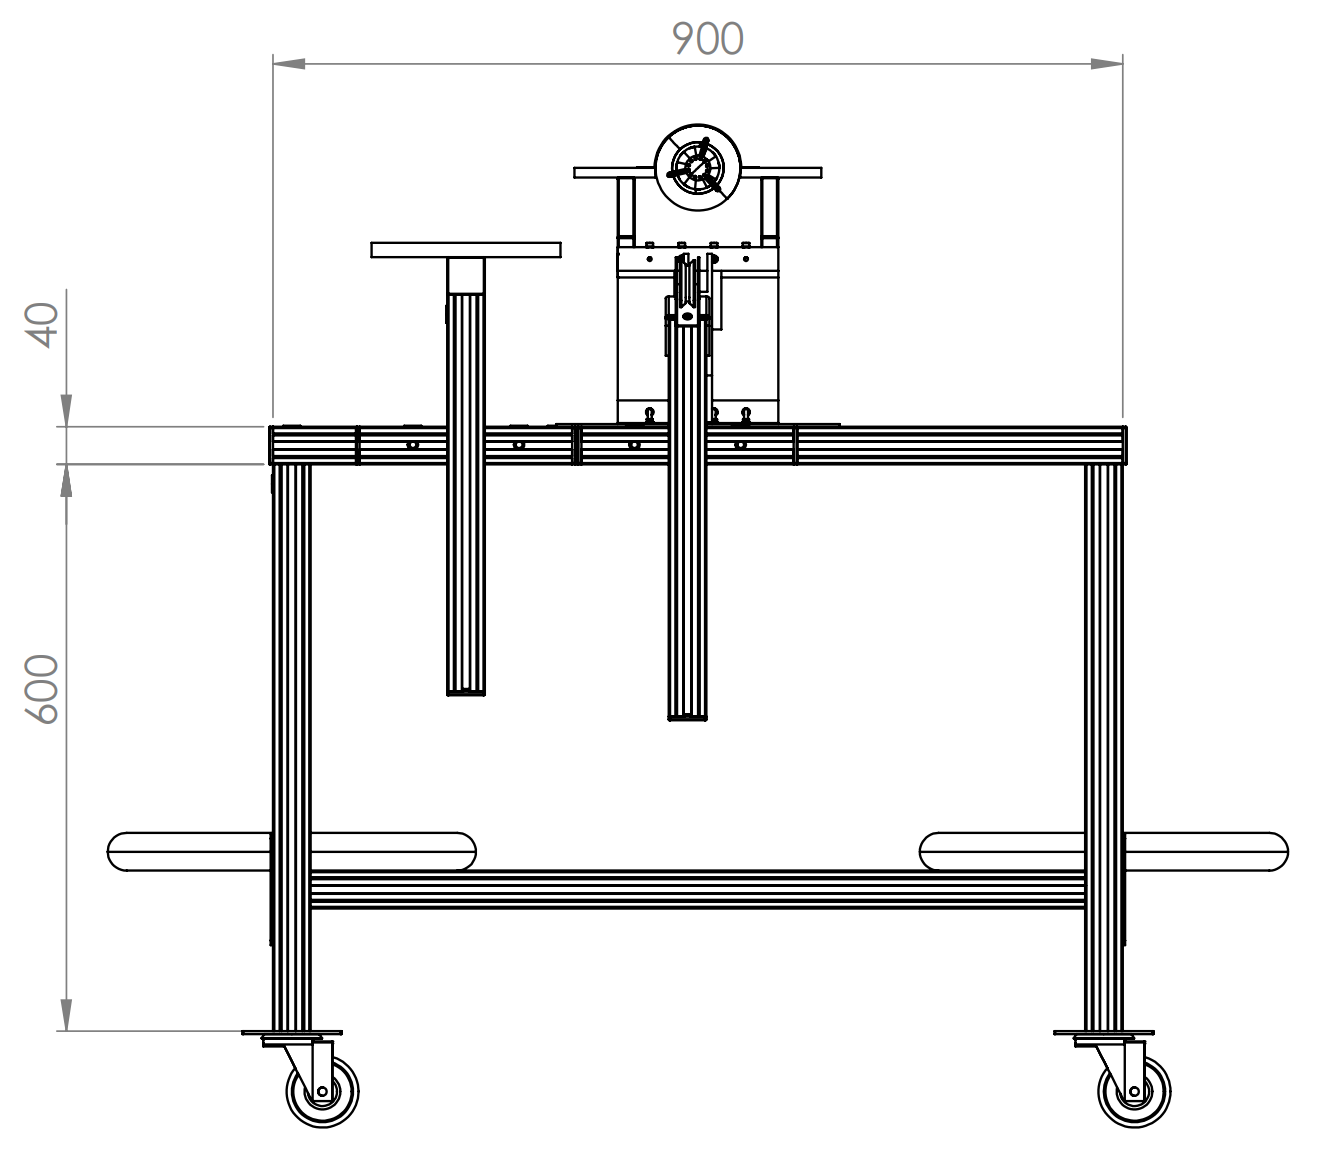
\includegraphics[width=.9\textwidth]{fig/test_bench_drawing.png}
        \caption{Blueprint (dimensions in mm)}
        \label{fig:test_bench!blueprint}
    \end{subfigure}

    \begin{subfigure}{.49\textwidth}
        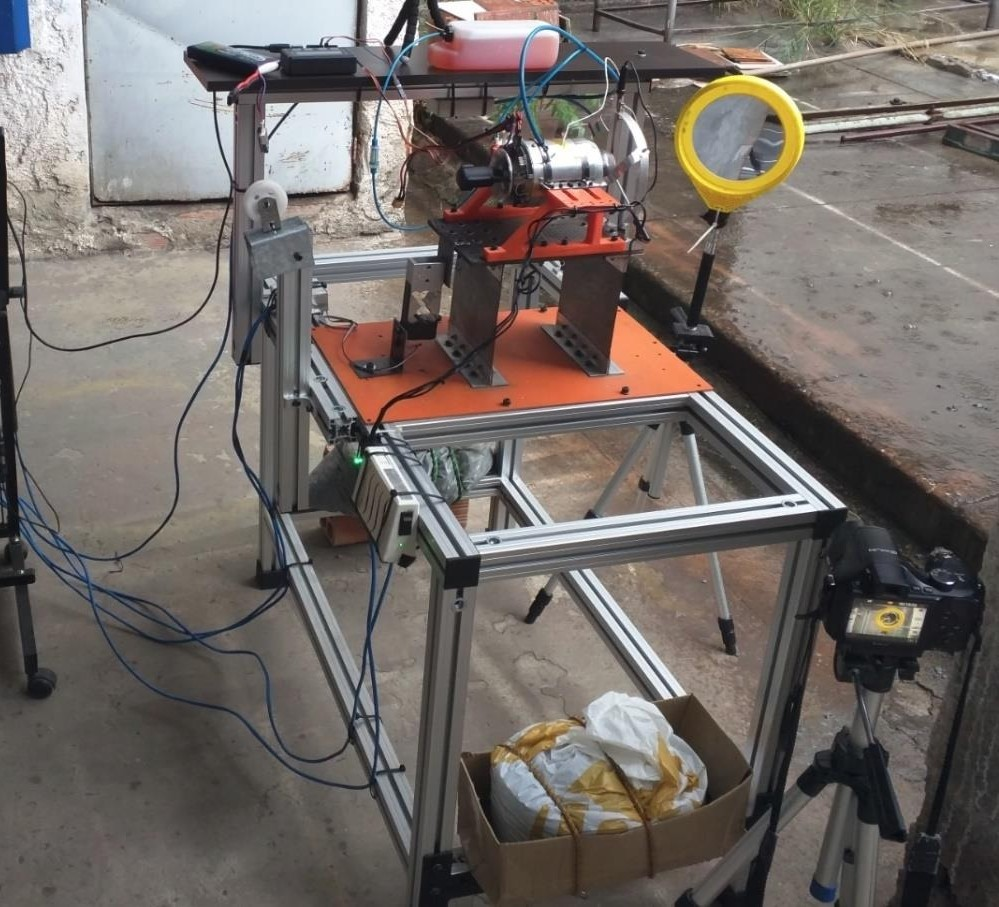
\includegraphics[width=.9\textwidth]{fig/engine_in_bench3.jpg}
        \caption{Picture with engine installed}
        \label{fig:test_bench!picture}
    \end{subfigure}
    \begin{subfigure}{.49\textwidth}
        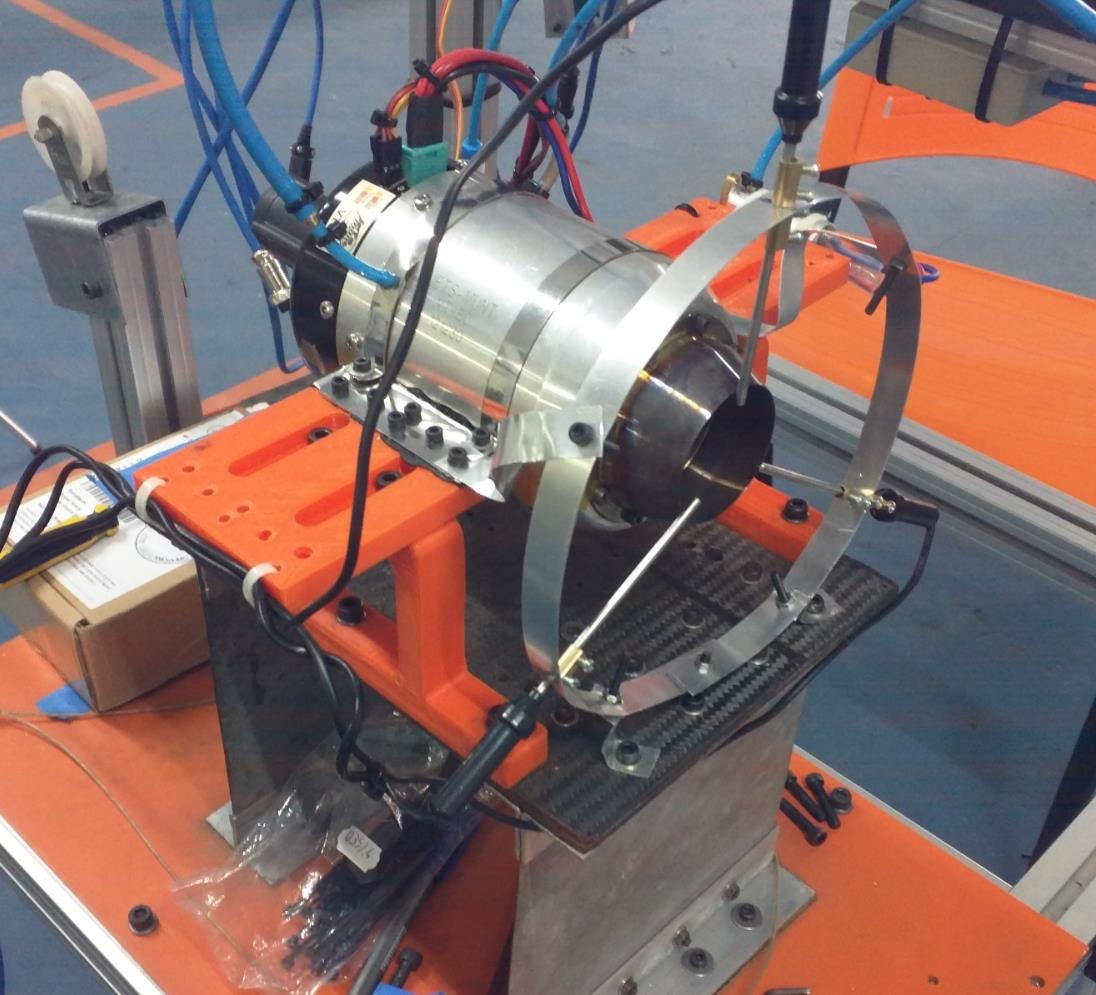
\includegraphics[width=.9\textwidth]{fig/engine_in_bench.jpg}
        \caption{Close up picture with engine installed}
        \label{fig:engine!closeup}
    \end{subfigure}
    \source{\cite{bolsoni}}
\end{figure}
\end{document}
